\documentclass[oneside,11pt, a4paper, footinclude=true, headinclude=true, cleardoublepage=empty]{scrbook}
\usepackage[linedheaders,parts,pdfspacing,dottedtoc]{classicthesis}
\usepackage{amsmath,amssymb}
\usepackage{amsthm}
\usepackage{acronym}
\usepackage[a4paper, hmargin={2.5cm, 2.5cm}, vmargin={2cm, 2cm}]{geometry}
\usepackage{eso-pic} % \AddToShipoutPicture
\usepackage{graphicx} % \includegraphics
\usepackage[utf8]{inputenc}
\usepackage[danish]{babel}
\usepackage{csquotes}
\usepackage{bookmark}
\usepackage[toc,page]{appendix}
\usepackage{longtable}
\usepackage{array}
\usepackage{multirow}
\usepackage{times}
\usepackage{lingmacros}
\usepackage{color, colortbl}
\usepackage{tabularx}
\usepackage{pdfpages}
\usepackage{footnote}
\definecolor{mygray}{rgb}{0.86,0.86,0.86}
\makesavenoteenv{tabular}
\makesavenoteenv{table}
\usepackage{hyperref}
\usepackage[backend=biber,defernumbers=true, style=authortitle]{biblatex}
\usepackage[multiple]{footmisc}
\definecolor{codegreen}{rgb}{0,0.6,0}
\definecolor{codegray}{rgb}{0.5,0.5,0.5}
\definecolor{codepurple}{rgb}{0.58,0,0.82}
\definecolor{backcolour}{rgb}{0.95,0.95,0.92}
\usepackage{listings}
\renewcommand{\lstlistingname}{Algoritme}
\usepackage{algorithm}
\usepackage[noend]{algpseudocode}
\makeatletter
\def\BState{\State\hskip-\ALG@thistlm}
\makeatother
\usepackage{xcolor}
\setboolean{@twoside}{false}
\newcommand{\overbar}[1]{\mkern 1.5mu\overline{\mkern-1.5mu#1\mkern-1.5mu}\mkern 1.5mu}
\usepackage{pgfplots}
\usepackage{tikz}
\usepackage{float}
\usepackage{relsize}
\renewcommand{\baselinestretch}{2.0}
\def\signed #1{{\leavevmode\unskip\nobreak\hfil\penalty50\hskip2em
  \hbox{}\nobreak\hfil(#1)%
    \parfillskip=0pt \finalhyphendemerits=0 \endgraf}}

    \newsavebox\mybox
    \newenvironment{aquote}[1]
      {\savebox\mybox{#1}\begin{quote}}
          {\signed{\usebox\mybox}\end{quote}}


\renewcommand{\cfttabpresnum}{} % get rid of "table"
\renewcommand{\cftfigpresnum}{}

\theoremstyle{definition}
\newtheorem{definition}{Definition}[section]
\theoremstyle{plain}
\newtheorem{theorem}{Sætning}[section]
\theoremstyle{lemma}
\newtheorem*{lemma}{Lemma}

\def \ColourPDF {Images/ku-farve.pdf}
\def \TitlePDF   {Images/ku-en.pdf}
\usepackage{minted}
\usemintedstyle{emacs}
\usepackage{keyval,kvoptions,fancyvrb,fvextra,upquote,ifthen,calc,ifplatform,pdftexcmds,etoolbox,xstring,lineno,framed,shellesc}
\subject{ 
  \vspace{3.5cm}
  \scriptsize{Matematiknoter til Matematik A og videregående} \\
  \Large{Matematik} \\}
\renewcommand{\baselinestretch}{1.5}
\title{
  \Huge{Matematik}\\
  \Large{... og hvad der kommer med}
}
\renewcommand*{\lstlistlistingname}{Code Listings}
\renewcommand*{\lstlistingname}{Code Listing}
\definecolor{gray}{gray}{0.5}
\colorlet{commentcolour}{green!50!black}

\colorlet{stringcolour}{red!60!black}
\colorlet{keywordcolour}{magenta!90!black}
\colorlet{exceptioncolour}{yellow!50!red}
\colorlet{commandcolour}{blue!60!black}
\colorlet{numpycolour}{blue!60!green}
\colorlet{literatecolour}{magenta!90!black}
\colorlet{promptcolour}{green!50!black}
\colorlet{specmethodcolour}{violet}
\newcommand*{\framemargin}{3ex}
\usepackage{dirtytalk}
\newcommand*{\literatecolour}{\textcolor{literatecolour}}
\usepackage{subcaption}
\newcommand*{\pythonprompt}{\textcolor{promptcolour}{{>}{>}{>}}}
\lstdefinestyle{mypython}{
%\lstset{
%keepspaces=true,
language=python,
showtabs=true,
tab=,
tabsize=2,
basicstyle=\ttfamily\footnotesize,%\setstretch{.5},
stringstyle=\color{stringcolour},
showstringspaces=false,
alsoletter={1234567890},
otherkeywords={\%, \}, \{, \&, \|},
keywordstyle=\color{keywordcolour}\bfseries,
emph={and,break,class,continue,def,yield,del,elif ,else,%
except,exec,finally,for,from,global,if,import,in,%
lambda,not,or,pass,print,raise,return,try,while,assert,with},
emphstyle=\color{blue}\bfseries,
emph={[2]True, False, None},
emphstyle=[2]\color{keywordcolour},
emph={[3]object,type,isinstance,copy,deepcopy,zip,enumerate,reversed,list,set,len,dict,tuple,xrange,append,execfile,real,imag,reduce,str,repr},
emphstyle=[3]\color{commandcolour},
emph={Exception,NameError,IndexError,SyntaxError,TypeError,ValueError,OverflowError,ZeroDivisionError},
emphstyle=\color{exceptioncolour}\bfseries,
%upquote=true,
morecomment=[s]{"""}{"""},
commentstyle=\color{commentcolour}\slshape,
%emph={[4]1, 2, 3, 4, 5, 6, 7, 8, 9, 0},
emph={[4]ode, fsolve, sqrt, exp, sin, cos,arctan, arctan2, arccos, pi,  array, norm, solve, dot, arange, isscalar, max, sum, flatten, shape, reshape, find, any, all, abs, plot, linspace, legend, quad, polyval,polyfit, hstack, concatenate,vstack,column_stack,empty,zeros,ones,rand,vander,grid,pcolor,eig,eigs,eigvals,svd,qr,tan,det,logspace,roll,min,mean,cumsum,cumprod,diff,vectorize,lstsq,cla,eye,xlabel,ylabel,squeeze},
emphstyle=[4]\color{numpycolour},
emph={[5]__init__,__add__,__mul__,__div__,__sub__,__call__,__getitem__,__setitem__,__eq__,__ne__,__nonzero__,__rmul__,__radd__,__repr__,__str__,__get__,__truediv__,__pow__,__name__,__future__,__all__},
emphstyle=[5]\color{specmethodcolour},
emph={[6]assert,yield},
emphstyle=[6]\color{keywordcolour}\bfseries,
emph={[7]range},
emphstyle={[7]\color{keywordcolour}\bfseries},
% emph={[7]self},
% emphstyle=[7]\bfseries,
literate=*%
{:}{{\literatecolour:}}{1}%
{=}{{\literatecolour=}}{1}%
{-}{{\literatecolour-}}{1}%
{+}{{\literatecolour+}}{1}%
{*}{{\literatecolour*}}{1}%
{**}{{\literatecolour{**}}}2%
{/}{{\literatecolour/}}{1}%
{//}{{\literatecolour{//}}}2%
{!}{{\literatecolour!}}{1}%
%{(}{{\literatecolour(}}{1}%
%{)}{{\literatecolour)}}{1}%
{[}{{\literatecolour[}}{1}%
{]}{{\literatecolour]}}{1}%
{<}{{\literatecolour<}}{1}%
{>}{{\literatecolour>}}{1}%
{>>>}{\pythonprompt}{3}%
,%
%aboveskip=.5ex,
frame=trbl,
%frameround=tttt,
%framesep=.3ex,
rulecolor=\color{black!40},
%framexleftmargin=\framemargin,
%framextopmargin=.1ex,
%framexbottommargin=.1ex,
%framexrightmargin=\framemargin,
%framexleftmargin=1mm, framextopmargin=1mm, frame=shadowbox, rulesepcolor=\color{blue},#1
%frame=tb,
backgroundcolor=\color{white},
breakindent=.5\textwidth,frame=single,breaklines=true%
%}
}
\lstset{style=mypython}
\addbibresource{references.bib}
\addbibresource{referenceszot.bib}
\lstdefinestyle{mypythoninline}{
style=mypython,%
basicstyle=\ttfamily,%
keywordstyle=\color{keywordcolour},%
emphstyle={[7]\color{keywordcolour}},%
emphstyle=\color{exceptioncolour},%
literate=*%
{:}{{\literatecolour:}}{2}%
{=}{{\literatecolour=}}{2}%
{-}{{\literatecolour-}}{2}%
{+}{{\literatecolour+}}{2}%
{*}{{\literatecolour*}}2%
{**}{{\literatecolour{**}}}3%
{/}{{\literatecolour/}}{2}%
{//}{{\literatecolour{//}}}{2}%
{!}{{\literatecolour!}}{2}%
%{(}{{\literatecolour(}}{2}%
%{)}{{\literatecolour)}}{2}%
{[}{{\literatecolour[}}{2}%
{]}{{\literatecolour]}}{2}%
{<}{{\literatecolour<}}{2}%
{<=}{{\literatecolour{<=}}}3%
{>}{{\literatecolour>}}{2}%
{>=}{{\literatecolour{>=}}}3%
{==}{{\literatecolour{==}}}3%
{!=}{{\literatecolour{!=}}}3%
{+=}{{\literatecolour{+=}}}3%
{-=}{{\literatecolour{-=}}}3%
{*=}{{\literatecolour{*=}}}3%
{/=}{{\literatecolour{/=}}}3%
%% emphstyle=\color{blue},%
}

\newcommand*{\pyth}{\lstinline[style=mypythoninline]}

\author{
  \Large{Sebastian Winkelmann}
}
\date{\today}


%DH: general comments: check commas and spelling. You can easily lose points if the writing comes across as sloppy, because reviewers might assume that the research was also sloppy.

\newenvironment{longlisting}{\captionsetup{type=listing}}{}
\begin{document}
\pagenumbering{roman}
\clearpage\maketitle
\thispagestyle{empty}
\tableofcontents
\pagenumbering{arabic}\part{Matematik A}
\part{Videregående}
%\chapter{Mængder og sæt}
Et sæt er en endelig eller uendelig mængde af objekter hvor rækkefølgen ingen vigtighed har og mulitiplicitet generelt ignoreres (modsat lister og multisæt). Medlemmer af en mængde kaldes for elementer og notationen $a\in A$ viser at $a$ er et element i sættet $A$. 

Store bogstaver ($A$, $B$, $X$, $Y$, osv) betegner mængder, mens små bogstaver ($a$, $b$, $x$, $y$, osv.) betegner elementer. Rækkefølgen af elementerne i et sæt er ligegyldig, således er $X=\left\{ 1,2,3\right\}$ og $Y=\left\{ 2,3,1\right\}$ lige med hinanden. 
Et sæt som intet indeholder kaldes tomt (\textbf{eng}: \textit{empty}, \textit{null} eller \textit{void}) og denoteres $\emptyset$, hvor $\emptyset = \{\}$.
\section{Prædefinerede sæt}
\textbf{Mængden af alle heltal} har bogstavet \textbf{Z} (eller $\mathbb{Z}$), hvor $\mathbb{Z}=\{\ldots, -2, -1, 0, 1, 2, \ldots\}$ (når udeladelsesprikker benyttes til sidst eller først, antyder det at den fortsætter \emph{uendeligt} i den retning).\\
\textbf{Mængden af alle positive tal (naturlige tal)} har bogstavet \textbf{N} (eller $\mathbb{N}$), hvor $\mathbb{N}=\{1,2,3,\ldots\}$. Således er et naturligt tal et positivt heltal.\\
\textbf{Mængden af alle reelle tal} har bogstavet \textbf{R} (eller $\mathbb{R}$), hvor $\mathbb{R}$ kan beskrive ethvert tal, mens $R^+$ beskriver ethvert positivt, og så videre.\\
\textbf{Mængden af rationelle tal} har bostavet \textbf{Q} (eller $\mathbb{Q}$) og er et reelt tal som kan udtrykkes som en kvotient af to heltal\[\frac{m}{n}\quad, \text{hvor } m,n\in \mathbb{Z}\]hvor $n$ naturligvis ikke må være nul ($n\neq 0$).\\
\textbf{Mængden af irrationelle tal} har ikke officielt noget bogstav (men \textbf{I} eller $\mathbb{I}$ kan benyttes) er ethvert reelt tal som ikke kan beskrives som en kvotient. Et sådan tal har (uendelige) ikke-periodiske decimaler. Eksempler på disse er $\sqrt{2}$, $\sqrt{3}$, $\sqrt[3]{2}$, $\pi$ og $e$.
\subsection{Kardinalitet \texorpdfstring{-- $|A|$}{|A|}}
Kardinaliteten (eller kardinaltallet) for en mængde $S$ er givet ved $|S|$, og betegner antallet af elementer i $S$. Det er her vigtigt at huske at en mængde også kun fungerer som ét element. Ved $A=\{1,2,\{3,4\},5\}$ vil det for $A$'s kardinaltal gælde at $|A|=4$.
\subsubsection{Eksempel}
Lad $D=\{n\in\mathbb{N}:n\leq 9\}, E=\{x\in\mathbb{Q}:x\leq9\}, H=\{x\in\mathbb{R}:x^2-2=0\}$ og $J=\{x\in\mathbb{Q}:x^2-2=0\}$.
\begin{enumerate}
    \item \textit{Beskriv mængden $D$ ved at opskrive dens elementer.}\\ $D=\{1,2,3,4,5,6,7,8,9\}$.
    \item \textit{Giv et eksempel på tre elementer som tilhører $E$ men ikke tilhører $D$.}\\$-2$, $8.9$, $1.5$.
    \item \textit{Beskriv mængden $H$ ved at opskrive dens elementer.}\\ $H=\{-\sqrt{2}, \sqrt{2}\}$.
    \item \textit{Beskriv sættet $J$ på en anden måde.}\\Ligningen har ingen løsninger indenfor de rationelle, hvorfor $J=\emptyset$.
    \item \textit{Bestem kardinaliteten for hvert sæt $D, H$ og $J$.}\\ $|D|=9$, $|H|=2$ og $|J|=0$.
\end{enumerate}
\section{Delmængder \texorpdfstring{-- $\subset$}{}}
Et sæt $A$ er en delmængde af $B$ hvis ethvert element af $A$ også tilhører $B$. Hvis $A$ er en delmængde af $B$, så skriver man $A\subseteq B$, hvorved $B$ er en supermængde af $A$: $A\supseteq B$. Således gælder det at $\mathbb{N}\subseteq \mathbb{Z}$, $\mathbb{Q}\subseteq \mathbb{R}$ og $\mathbb{Q}\subseteq \mathbb{R}$. Da $\mathbb{Q}\subseteq \mathbb{R}$ og $\mathbb{R}\subseteq \mathbb{C}$, følger det at $\mathbb{Q}\subseteq \mathbb{C}$. Det gælder desuden at hver mængde er dets eget delmængde. Det gælder dog at $\mathbb{Z}\subsetneq \mathbb{N}$.
\section{Mængdeoperatorer}

\subsection{Foreningsmængde \texorpdfstring{-- $\cup$}{}}
Foreningen af to mængder $A$ og $B$ skrives $A\cup B$ (\textbf{eng}: \textit{union}; \textbf{latex}: \texttt{cup}), og er det sæt af elementer som tilhører $A$ eller $B$; altså \[A\cup B = \left\{ x:x\in A \lor x\in B\right\}\]
hvor \textit{eller} ($\lor$) betyder at et element i $A\cup B$ både kan tilhøre $A$ og $B$. Således vil $x$ være i $A\cup B$ hvis
\begin{enumerate}
    \item $x$ er i $A$
    \item $x$ er i $B$
    \item $x$ er i både $A$ og $B$
\end{enumerate}
Et Venn-diagram kan bruges til at illustrere dette på. Se figur \ref{fig:foreningvenn}.
\begin{figure}[H]
    \centering
    \includegraphics[width=0.4\textwidth]{billeder/Acrobat_h4xoc29CTB.png}
    \caption{Venn-diagram, hvor det tonede område betegner $A\cup B$}
    \label{fig:foreningvenn}
\end{figure}
\subsection{Fællesmængde \texorpdfstring{-- $\cap$}{}}
Fællesmængden af to mængder $A$ og $B$ skrives $A\cup B$ (\textbf{eng}: \textit{intersection}; \textbf{latex}: \texttt{cap}), og er det sæt af elementer som både tilhører $A$ og $B$; altså \[A\cap B=\{ x:x\in A \land x\in B\}\]
Et Venn-diagram kan bruges til at illustrere dette på. Se figur \ref{fig:fellesvenn}.
\begin{figure}[H]
    \centering
    \includegraphics[width=0.4\textwidth]{billeder/Acrobat_bHAl8Wuekv.png}
    \caption{Venn-diagram, hvor det tonede område betegner $A\cap B$}
    \label{fig:fellesvenn}
\end{figure}
\subsubsection{Disjunkt}
Hvis to mængder ikke har nogle elementer tilfælles siges de at være disjunkt, altså adskilte. For to disjunkte mængder gælder det at \[A\cap B = \emptyset\]
Sammenhængen mellem foreningsmængde og fællesmængde er\[A\cap B\subseteq A\cup B\]
\subsection{Mængdedifferens og relativ komplementærmængde \texorpdfstring{$-$ eller $\setminus$}{}}
Differensen $A-B$ af to mængder $A$ og $B$ (også skrevet $A\setminus B$) er defineret som\[ A-B=\{x:x\in A\,\land x\notin B\}\]Et Venn-diagram kan bruges til at illustrere dette på. Se figur \ref{fig:differensvenn}.
\begin{figure}[H]
    \centering
    \includegraphics[width=0.4\textwidth]{billeder/Acrobat_mR0KSCJDtQ.png}
    \caption{Venn-diagram, hvor det tonede område betegner $A-B$}
    \label{fig:differensvenn}
\end{figure}
\textit{Mængdedifferensen kaldes også for \textbf{den relative komplementærmængde}. (læs mere om komplementærmængder i nedenunder)}
\subsection{Komplementærmængde\texorpdfstring{ -- $\overline{A}$}{}}
Komplementærmængden $\overline{A}$ af $A$ er mængdedifferensen af universalmængden $U$ og $A$; altså\[\overline{A}=\{x:x\in U \land x\notin A\}\]Et Venn-diagram kan bruges til at illustrere dette på. Se figur \ref{fig:complementvenn}.
\begin{figure}[H]
    \centering
    \includegraphics[width=0.4\textwidth]{billeder/Acrobat_p0XoSIqOY7.png}
    \caption{Venn-diagram, hvor det tonede område betegner $\overline{A}$}
    \label{fig:complementvenn}
\end{figure}
\subsection{Mange mængder}
Ønsker man at behandle flere mængder bør man indeksere disse. Har man $n$ sæt, $A_1, A_2, \ldots, A_n$, så vil disses \textbf{foreningsmængde} være $A_1\cup A_2\cup \ldots \cup A_n$, eller bare $\bigcup_{i=1}^n A_i$ og er defineret som enhver værdi som befinder sig i sættene\[\bigcup_{i=1}^n A_i = \{x:x\in A_i \text{ for en } i, 1\leq i\leq n\}\]
\textbf{Fællesmængden} for disse er udtrykt ved $A_1\cap A_2\cap\ldots\cap A_n$ eller $\bigcap_{i=1}^n A_i$ og er defineret som enhver værdi som er i alle sættene\[\bigcap_{i=1}^n A_i=\{x:x\in A_i \text{ for alle } i, 1\leq i\leq n\}\]
\section{Partition og deling}
Hvis to mængders fællesmængde er tom, da siges de at være disjunkte. Hvis en samling\footnote{En samling er en mængde som består af mængder.} $\mathcal{S}$ er en delmængde af mængden $A$ er den \textbf{parvist disjunkt} hvis et vilkårligt delmængde-par som tilhører $\mathcal{S}$ er disjunkt.\par\textbf{Eksempel.} Lad $A=\{1,2,\ldots,7\}$, $B=\{1,6\}$, $C=\{2,5\}$, $D=\{4,7\}$ og $S=\{B,C,D\}$. Herved er $S$ en parvis disjunkt samling af delmængder af $A$ da\[B\cap C=B\cap D=C\cap D=\emptyset\]\par
En \textbf{partition} af en mængde $A$ er en samling $\mathcal{S}$ af ikke-tomme delmængder af $A$ således at hvert element af $A$ tilhører præcist én delmængde i $\mathcal{S}$. Altså vil en partition af $A$ være den samling $\mathcal{S}$ af delmængder af $A$ som tilfredsstiller
\begin{enumerate}
    \item $X\neq\emptyset$ for hvert sæt $X\in\mathcal{S}$
    \item for hver par af mængder $X,Y\in\mathcal{S}$, vil enten $X=Y$ eller $X\cap Y=\emptyset$
    \item $\bigcup_{X\in\mathcal{S}}X=A$
\end{enumerate}\par\textbf{Eksempel.} Mængden af reelle tal $\mathbb{R}$ kan partitioneres/deles op i tre mængder: Mængden af alle positive, reelle tal ($\mathbb{R}^+$); Mængden af alle negative, reelle tal ($\mathbb{R}^-$); Mængden som består af nul ($\{0\}$). Således at $S_\mathbb{R}=\{R^-, \{0\}, R^+\}$.
\section{Jan Philip Solovejs forelæg 02-09}
Der er forskel på tal. Der er nemme tal (naturlige tal; $\mathbb{N}=\lbrace0,1,2,\ldots\rbrace$), men også algebraiske tal og ikke-matematiske tal (som ikke kan bestemmes ved matematiske beregninger, men er afhængige af målinger). De hele tal ($\mathbb{Z}=\lbrace\ldots,-1,0,1,\ldots\rbrace$), de rationelle tal ($\mathbb{Q}=\lbrace\frac{p}{q}:p\in \mathbb{Z},q\in\mathbb{N}\rbrace$), og de irrationelle tal.

\begin{proof}{Hvis $a$ er ulige: $a=2n-1$.}
\begin{lemma}Hvis $a\in\mathbb{N}$ og $a$ er ulige, da er $a^2$ ulige.\end{lemma}
Vi ved at $a^2=(2n-1)^2=4n^2+1-4n=2(2n^2-2n)+1$, altså vil produktet af ulige tal give et ulige tal. Det samme gælder for primtalsfaktorisering, hvor alle lige tal faktoriseres med 2.
\end{proof}

\begin{proof}{$\sqrt{2}\notin\mathbb{Q}$}
Antag at $\sqrt{2}=\frac{n}{m}\implies\sqrt{2m}=n\implies2m^2?n^2\implies n\text{ er lige}$, hvor $\frac{n}{m}$ er uforkortelige. Altså $n=2p\text{ hvis }p\in\mathbb{N}$.\\$2m^2=n^2=(2p)^2=4p^2\implies m^2=2p^2$, hvorved både $m$ og $n$ er lige, hvorfor $\sqrt{2}$ må være et irrationelt tal.
\end{proof}
Reelle tal $\mathbb{R}$ er tal, der kan tilnærmes med rationelle tal. Notationen for mængder er ved åbent interval $$]a,b[=(a,b)=\lbrace x\in\mathbb{R}|a<x<b\rbrace$$mens lukkede er $$[a,b]=\lbrace x\in\mathbb{R}|a\leq x\leq b\rbrace$$Den numeriske værdi er talværdien, eller den absolutte værdi $|a|=\begin{cases}
    \,\,\,\,\,a, \,\, a\geq0\\
    -a, \,\,a<0
  \end{cases}$
  
Lige meget hvilket reelt tal man vælger, vil der altid være et naturligt tal som er større. <- Arkimedes princip.

\begin{proof}{$a,b\in\mathbb{R}$ og $a<b$ da vil intervallet $(a,b)$ indeholde både rationelle og irrationelle tal, lige meget hvor småt, altså at $(a,b)\cap \mathbb{Q}\neq \emptyset$}, mens $(a,b)\cap(\mathbb{R}\setminus\mathbb{Q}\neq\emptyset$

\end{proof}
\textbf{Fuldstændighedsegenskaben:} Hvis $A\subseteq\mathbb{R}$ og $A\subseteq(-\infty,b]$ $b\in\mathbb{R}$. Enhver mængde $A$ som er indeholdt i $(-\infty,b)$ fra et eller andet $b$ har en mindste øvre grænse, altså supremum, $\text{sup}A$. I $\text{sup}(-2,3)=3$ og $\text{sup}(-2,3]=3$ <- her et ekstremum.

En metode til at finde rødder i polynomier er ved at bryge polynomiers division: Man kan dividere roden ud, hvis man kender en anden rod. Eksempel: $\frac{x^2+5x+7}{x+2}$

\subsection{Komplekse tal}Vi indfører $\sqrt{-1}=i$ løser $x^2+1=0\implies x=\pm i$. Definition: $i^2=-1$. Når man ganger to komplekse tal foregår det ved $(2+3i)(1+i)=2(1+i)+3i(1+i)=2+2i+3i+3i^2=2+5i-3=-1+5i$. Mængden af komplekse tal er givet ved \begin{equation}
    \mathbb{C}=\{a+ib|a,b\in\mathbb{R}\}
\end{equation}
\chapter{Reelle og komplekse tal}
\section{Polynomier og polynomiedivision}
Et $n$-te gradspolynomium er udtrykt på formen\begin{equation}
    P(x)=a_nx^n+a_{n-1}x^{n-1}+a_{n-2}x^{n-2}+\cdots+a_2x^2+a_1x+a_0
\end{equation}Ved polynomiedivision deler man to polynomier med hinanden. \subsection{Eksempel}For at dele $P(x)=2x^4+4x^3-3x^2+x+4$ med $Q(x)=x^2-2x+4$ skal vi gøre som med et normalt divisionsstykke:\begin{equation}
    2x^4+4x^3-3x^2+x+4 : x^2-2x+4
\end{equation}For at få det til at passe med det største led af divindenden ganger vi divisoren med $2x^2$. Således er divisoren nu $2x^4-4x^3+8x^2$. Nu trækker vi divisoren fra dividenden:\begin{align}
    2x^4+4x^3&-3x^2+x+4\\
    -(2x^4-4x^3&+8x^2)\,=\\
    8x^3&-11x^2+x+4
\end{align}
Næste led, $8x^3$, kan vi få til at gå op i $x^2$ præcis $8x$ gange. Således har vi at divisoren er $8x\cdot(x^2-2x+4)=8x^3-16x^2+32x$, som vi trækker fra divindenden:\begin{align}
    8x^3-11x^2&+x+4\\
    -(8x^3-16x^2&+32x)\,=\\
    5x^2&-31x+4
\end{align}
Næste led! $5x^2$ går op i $x^2$ 5 gange, så
\begin{align}
    5x^2-31x&+4\\
    -(5x^2-10x&+20)\,=\\
    -21x&-16
\end{align}
Den \textit{ufuldstændige} kvotient $K(x)$ (uden resten $R(x)$) er hermed summen af de tal vi har brugt:$$2x^2+8x+5$$Her er resten (11), altså der hvor vi ikke længere kan bruge det største led i divisoren. Altså er \begin{equation}
    2x^4+4x^3-3x^2+x+4=(2x^2+8x+5)(x^2-2x+4)+(21x-16)
\end{equation}
Når graden af $P(x)$ er mindre end $Q(x)$ vil $K(x)=0$ og $R(x)=P(x)$.\\Et tal $a$ er en rod i polynomiet $P(x)$ hvis og kun hvis $P(x)$ er delelig med $x-a$.
\subsection{Rødder}

\section{Reelle tals komplethed}
En delmængde $A$ af $\mathbb{R}$ kaldes \textit{opad begrænset} hvis der findes et tal $b$ som er større eller lig med alle andre elementer i $A$. Dette $b$ kaldes for et \textbf{supremum} til $A$ hvis $b$ er mindre end alle andre supremer.\subsection{Komplethedsprincippet}Enhver ikke-tom, opad begrænset delmængde $A$ af $\mathbb{R}$ har et supremum.\\Derudover har enhver ikke-tom, nead begrænset delmængde $B$ af $\mathbb{R}$ en infimum.
\section{Komplekse tal}
Vi ved at den imaginære enhed er defineret ved $i^2=-1$, samt at et komplekst tal udtrykkes på formen $z=a+ib$, hvor $a$ og $b$ er reelle tal, men $a$ betegner den reelle del ($a=\text{Re}(z)$) og $b$ betegner den imaginære del ($b=\text{Im}(z)$). Sum og differens findes let, når $z=a+ib$ og $w=c+id$
\begin{equation}
    z+w=(a+c)+i(b+d)
\end{equation}
\begin{equation}
    z-w=(a-c)+i(b-d)
\end{equation}
Hvorimod multiplikation findes ved 
\begin{equation}
    z\cdot w=(ac-bd)+i(ad+bc)
\end{equation}
Og division er givet ved 
\begin{equation}
    \frac{z}{w}=\frac{ac+bd}{c^2+d^2}+i\frac{bc-ad}{c^2+d^2}
\end{equation}
Og den inverse er givet ved 
\begin{equation}
    z^{-1}=\frac{a}{a^2+b^2}-i\frac{b}{a^2+b^2}
\end{equation}
Ved \textbf{konjugation} bliver der vendt fortegn for andet led, hvilket kan opfattes som en spejling af $z$ om den reelle plan. Her er yderligere regneregler, blot for konjugation:
\begin{align}
    \overline{z}+\overline{w}&=\overline{z+w}\\
    \overline{z}-\overline{w}&=\overline{z-w}\\
    \overline{z}\,\,\,\overline{w}&=\overline{zw}\\
    \frac{\overline{z}}{\overline{w}}&=\overline{\left(\frac{z}{w}\right)}
\end{align}
\subsection{Geometrisk signifikans}
Komplekse tal kan opfattes geometrisk på koordinatsystemer. Enten i form af en reel $x$-akse og en imaginær $y$-akse, eller på polærform, hvor der vil være et argument ($\text{Arg}(z)=\theta$) og et modulus ($|z|=r$). Her er koefficienterne givet ved $a=r\cdot\cos{\theta}$ og $b=r\cdot\sin{\theta}$ -- hvor $r=\sqrt{a^2+b^2}$ og $\tan{\theta}=\frac{b}{a}$.\\
Summen kan geometrisk observeres som en vektorsum, med parallelogrammet. 
\begin{theorem}{Geometrisk fortolkning af produkt af komplekse tal (3.2.3).}
$z_1=r_1(\cos{\theta_1}+i\sin{\theta_1})$ samt $z_2=r_2(\cos{\theta_2}+i\sin{\theta_2})$.\begin{align}
    z_1z_2&=r_1r_2\left(\cos{(\theta_1+\theta_2)}+i\sin{(\theta_1+\theta_2)}\right)
\end{align}
\end{theorem}Dette kan man (ifølge Euler) omforme til eksponentialfunktion. Læs \ref{eks}.
\subsection{Enhedscirklen}
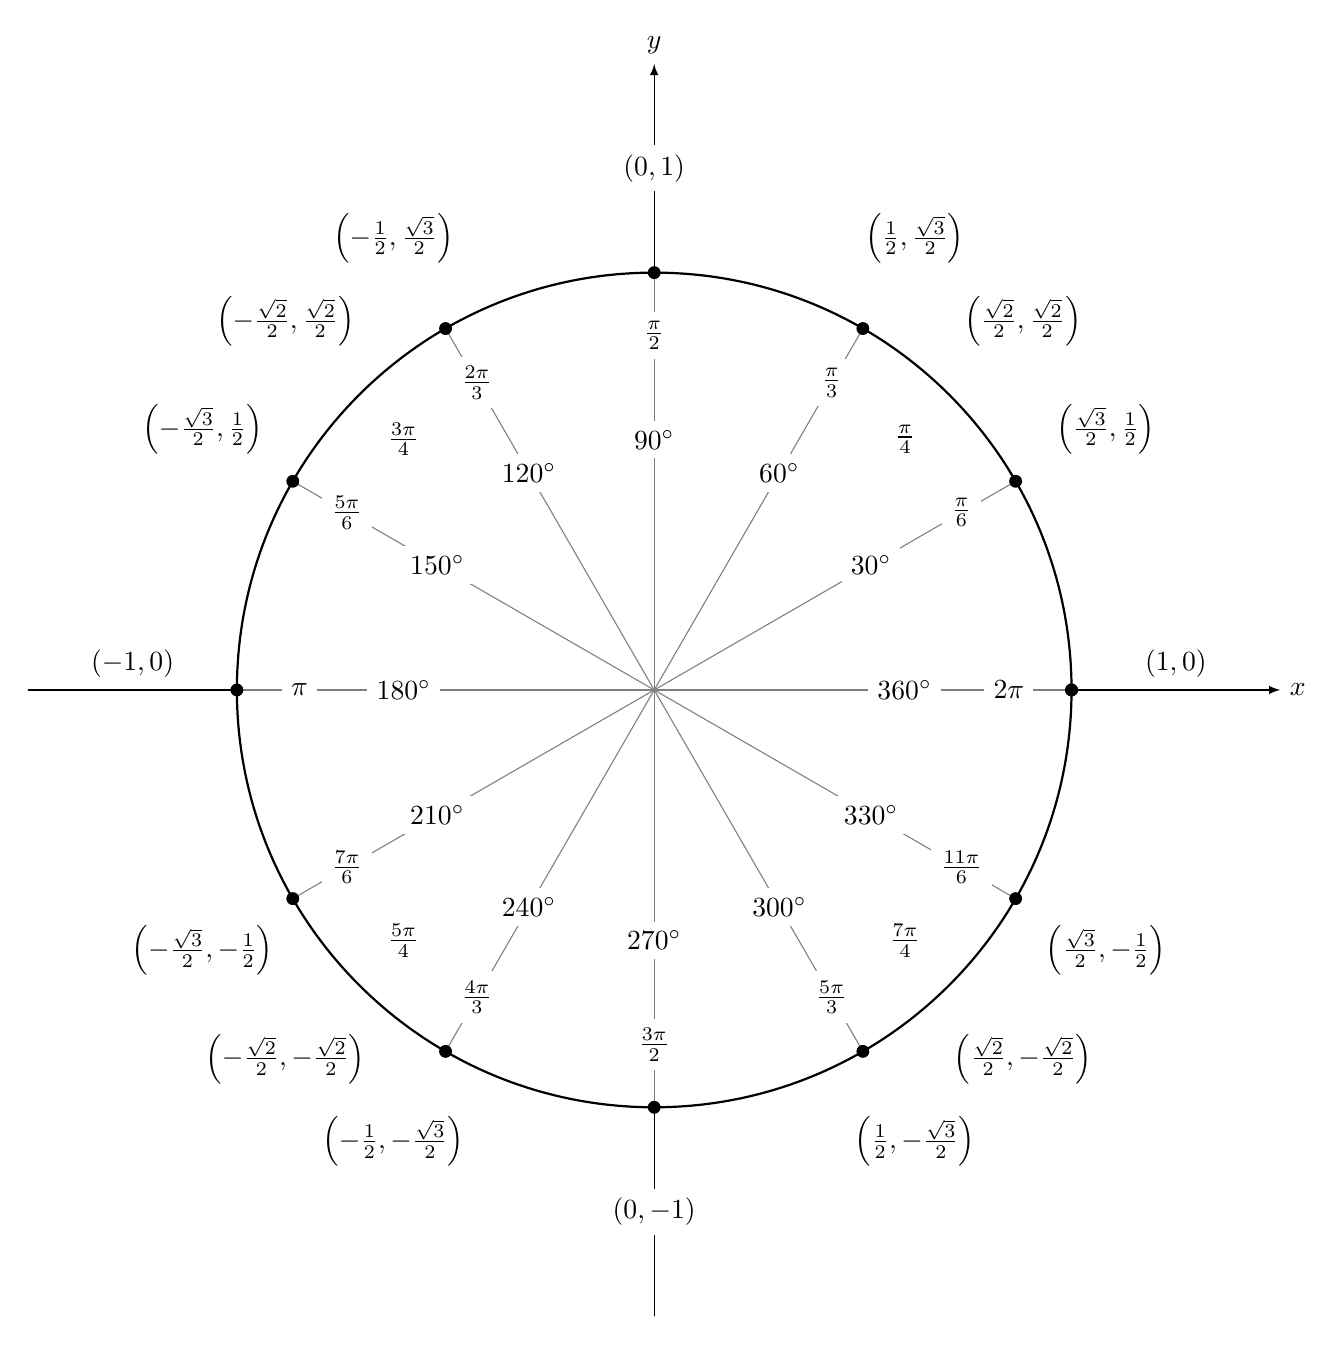
\begin{tikzpicture}[scale=5.3,cap=round,>=latex]
        % draw the coordinates
        \draw[->] (-1.5cm,0cm) -- (1.5cm,0cm) node[right,fill=white] {$x$};
        \draw[->] (0cm,-1.5cm) -- (0cm,1.5cm) node[above,fill=white] {$y$};

        % draw the unit circle
        \draw[thick] (0cm,0cm) circle(1cm);

        \foreach \x in {0,30,...,360} {
                % lines from center to point
                \draw[gray] (0cm,0cm) -- (\x:1cm);
                % dots at each point
                \filldraw[black] (\x:1cm) circle(0.4pt);
                % draw each angle in degrees
                \draw (\x:0.6cm) node[fill=white] {$\x^\circ$};
        }

        % draw each angle in radians
        \foreach \x/\xtext in {
            30/\frac{\pi}{6},
            45/\frac{\pi}{4},
            60/\frac{\pi}{3},
            90/\frac{\pi}{2},
            120/\frac{2\pi}{3},
            135/\frac{3\pi}{4},
            150/\frac{5\pi}{6},
            180/\pi,
            210/\frac{7\pi}{6},
            225/\frac{5\pi}{4},
            240/\frac{4\pi}{3},
            270/\frac{3\pi}{2},
            300/\frac{5\pi}{3},
            315/\frac{7\pi}{4},
            330/\frac{11\pi}{6},
            360/2\pi}
                \draw (\x:0.85cm) node[fill=white] {$\xtext$};

        \foreach \x/\xtext/\y in {
            % the coordinates for the first quadrant
            30/\frac{\sqrt{3}}{2}/\frac{1}{2},
            45/\frac{\sqrt{2}}{2}/\frac{\sqrt{2}}{2},
            60/\frac{1}{2}/\frac{\sqrt{3}}{2},
            % the coordinates for the second quadrant
            150/-\frac{\sqrt{3}}{2}/\frac{1}{2},
            135/-\frac{\sqrt{2}}{2}/\frac{\sqrt{2}}{2},
            120/-\frac{1}{2}/\frac{\sqrt{3}}{2},
            % the coordinates for the third quadrant
            210/-\frac{\sqrt{3}}{2}/-\frac{1}{2},
            225/-\frac{\sqrt{2}}{2}/-\frac{\sqrt{2}}{2},
            240/-\frac{1}{2}/-\frac{\sqrt{3}}{2},
            % the coordinates for the fourth quadrant
            330/\frac{\sqrt{3}}{2}/-\frac{1}{2},
            315/\frac{\sqrt{2}}{2}/-\frac{\sqrt{2}}{2},
            300/\frac{1}{2}/-\frac{\sqrt{3}}{2}}
                \draw (\x:1.25cm) node[fill=white] {$\left(\xtext,\y\right)$};

        % draw the horizontal and vertical coordinates
        % the placement is better this way
        \draw (-1.25cm,0cm) node[above=1pt] {$(-1,0)$}
              (1.25cm,0cm)  node[above=1pt] {$(1,0)$}
              (0cm,-1.25cm) node[fill=white] {$(0,-1)$}
              (0cm,1.25cm)  node[fill=white] {$(0,1)$};
    \end{tikzpicture}
    $x=\cos{\theta},\quad y=\sin{\theta}$
\subsection{Algebraiske egenskaber}
\begin{enumerate}
    \item \textbf{Kommutative lov} -- $z_1+z_2=z_2+z_1$ og $z_1z_2=z_2z_1$
    \item \textbf{Associative lov} -- $(z_1+z_2)+z_3=z_1+(z_2+z_3)$, osv.
    \item \textbf{Distributive lov} -- $z_1(z_2+z_3)=z_1z_2+z_1z_3$
    \item \textbf{Nul- og enhedselement} -- $z_1+0=z_1$ og $z_1\cdot1=z_1$
    \item \textbf{Modsatte tal} -- for hvert komplekst tal $z$, findes der et komplekst tal $-z$ hvor $z+(-z)=0$
    \item \textbf{Inverse tal} -- for hvert komplekst tal $z\neq0$, findes der et komplekst tal $w$ hvor $zw=1$
\end{enumerate}
\subsection{Trekantsuligheden}
Ved komplekse tal $z$ og $w$ vil der gælde at \begin{equation}
    |x+w|\leq|z|+|w|
\end{equation}
\section{Den Komplekse Eksponentialfunktion}\label{eks}
Et komplekst tal $z=a+ib$ kan udtrykkes\begin{equation}
    e^z=e^a(\cos{b}+i\sin{b})
\end{equation}hvor $e^z$ er et komplekst tal med modulus $e^a$ og argumentet $b$. Der gælder desuden at $z=re^{i\theta}$.
\section{$n$-te rødder}
\begin{theorem}{$n$-te rødder af et komplekst tal.}
$z\in\mathbb{C}$, hvor at $w\in\mathbb{C}$ er en $n$-te rod af $z$ hvis $w^n=z$. Alle disse rødder kan findes således, når $z=re^{i\theta}$. Da har vi\begin{align}
    w_0&=r^{\frac{1}{n}}e^{i\frac{\theta}{n}}\\
    w_1&=r^{\frac{1}{n}}e^{i\left(\frac{\theta}{n}+\frac{2\pi}{n}\right)}\\
    &\ldots\\
    w_{n-1}&=r^{\frac{1}{n}}e^{i\left(\frac{\theta}{n}+\frac{2\pi(n-1)}{n}\right)}
\end{align}
Så vil der altså gælde at $z=re^{i\theta}$ præcist har $n$ $n$-rødder givet ovenover.
\end{theorem}
\section{Komplekse 2.gradsligninger}
Vi har en ligning \begin{equation}
    az^2+bz+c=0,\,\quad\text{ hvor }a\neq0
\end{equation}Rødderne er givet ved \begin{equation}
    \frac{-b\pm i\sqrt{4ac-b^2}}{2a}
\end{equation}
Rødder vil blot være hinandens konjugerede.
\subsection{Algebraens fundamentalsætning}
Hvis $p(z)=c_hz^n+\ldots+c_1z+c_0,c_n\neq0$, da findes $r_1,\ldots,r_n\in\mathbb{C}$ så $p(n)=c_n(z-r_1)(z-r_2)\cdots(z-r_n)$.

Se desuden på et polynomium $P(x)$ og et tal $\alpha$. Vi kan dividere disse, og få en kvotient og rest:$$P(x)=(x-\alpha)\cdot Q(x)+r$$hvor der gælder at $\alpha$ er rod i $P(x)$ $\iff$ $r=0$.
\chapter{Konvergens, følger, kontinuitet og grænser}
En følge er en uendelig sekvens af tal\begin{equation}
    \{a_n\}=a_1,a_2,a_3,\ldots,a_n,\ldots
\end{equation}Man bruger notationen $\{a_n\}$ for en følge, for eksempel\begin{align*}
    \{n^2\}&=1,4,9,16,25,36,49,\ldots,a^n,\ldots\\
    \{1/n\}&=1,\frac{1}{2},\frac{1}{3},\frac{1}{4},\frac{1}{5},\ldots,\frac{1}{n},\ldots\\
    \{\cos{n}\}&=\cos{1},\cos{2},\cos{3},\ldots,\cos{n},\ldots\\
    \{a_n\}&=a_1,a_2,a_3,a_4,\ldots,a_n,\ldots
\end{align*}
Man kan desuden angive det ønskede interval (hvis det er forskellig for $[n,\infty)$  ):$$\{a_n\}_{n=z}^\infty$$
\section{Konvergens af følger}
Talfølger kan enten gå mod et bestemt tal, eller fortsætte i det uendelige. I\begin{align}
    \left\{\frac{n}{n-1}\right\}&=0,\frac{1}{2},\frac{2}{3},\frac{3}{4},\frac{4}{5},\ldots,\frac{n}{n-1},\ldots\label{eq:conv}\\
    \{n^2\}&=1,4,9,16,\ldots,n^2,\ldots\label{eq:nonconv}
\end{align}
er det kun (\ref{eq:conv}) som rent faktisk går mod et tal (her tallet 1), mens (\ref{eq:nonconv}) blot stiger til et større tal hver for hver gang. Her siger vi at \textbf{\ref{eq:conv} konvergerer mod grænseværdien 1}, mens \textbf{\ref{eq:nonconv} divergerer}.
\begin{definition}{Konvergens af følge}
Følgen $\{a_n\}$ konvergerer mod tallet $a$ når der for ethvert reelt tal $\epsilon>0$ findes et tal $N\in\mathbb{N}$, således at $|a_n-a|<\epsilon$ for alle $n\geq N$. I så fald\begin{equation}
    \lim_{n\to\infty}a_n=a
\end{equation}En følge som konvergerer mod et tal, kaldes \textit{konvergent}, mens en følge som ikke konvergerer kaldes \textit{divergent}. Eller skrevet på en anden måde$$\forall\epsilon>0\exists N\in\mathbb{N}:n\geq N\implies|a_n-a|<\epsilon$$\end{definition}
Altså vil der være konvergens når man for afstanden $|a_n-n|$ kan vælge et tilstrækkelig stort $n$, således at afstanden bliver mindre.\\ Andre skrivemåder benyttes iøvrigt også$$a_n$$$$(a_n)$$\\
\begin{enumerate}
    \item Hvis $\{a_n\}$ er konvergent så er grænseværdien entydig!
    \item Hvis $\{a_n\}$ er konvergent så er $\{a_n|n\in\mathbb{N}\}$ begrænset
    \item ALLE periodiske funktioner divergerer
\end{enumerate}
Der findes voksende og aftagende talfølger, altså hhv. $a_{n+1}>a_n$ og $a_{n+1}<a_n$, i så fald er den desuden monoton. Er den samme talfølge begrænset, da er den konvergent. \\
\textbf{Supremumsegenskaben ved $\mathbb{R}$}: Enhver ikke-tom begrænset delmængde $A\subseteq\mathbb{R}$ har en mindste øvre grænse (supremum).
\section{Grænseværdier}
Når grænseværdien eksisterer skriver vi\begin{equation}
    \lim_{n\to\infty}a_n=a,\quad a_n\to a\text{ for } n\to\infty
\end{equation}
\begin{theorem}Antag at $\{a_n\}$ og $\{b_n\}$ er konvergente med grænseværdi $a,b$, da gælder \begin{align*}
    a_n\pm b_n&\to a\pm b\text{     for } n\to\infty\\
    a_nb_n&\to ab\text{     for } n\to\infty\\
\end{align*}\end{theorem}

\section{Kontinuerlige funktioner}
\begin{definition}{\textbf{Kontinuitet}}
En funktion $f$ er \textit{kontinuert} i et punkt $a\in D_f$ når følgende gælder: For enhver $\epsilon>0$ findes der en $\delta>0$ så når $x\in D_f$ og $|x-a|<\delta$, så er $|f(x)-f(a)|<\epsilon$. Vi kan altså få afstanden mellem $f(x)$ og $f(a)$ mindre end $\epsilon$ ved at kræve at afstanden mellem $x$ og $a$ er mindre end $\delta$.
\end{definition}
\begin{theorem}
Antag at $f$ og $g$ er kontinuerte i punktet $a$. Da vil funktionerne $f + g$, $f - g$ og $f\cdot g$ også være kontinuerte i $a$. Hvis $g(a) \neq0$ vil $\frac{f}{g}$ også være kontinuert i $a$.
\end{theorem}
\begin{theorem}
Antag at $f$ og $g$ er kontinuerte i punktet $a$ og $f$ i punktet $g(a)$. Da er den sammensatte funktion $h(x)=f[g(x)]$ også kontinuert i punktet $a$.
\end{theorem}
\begin{theorem}{Skæringssætningen}
Når en kontinuert funktion $f$ går fra plus til negativ værdi, da vil $f$ på et eller andet punkt være lig 0. Antag at $f:[a,b]\rightarrow\mathbb{R}$ er en kontinuert funktion hvor $f(a)$ og $f(b)$ har modsat fortegn. Da findes der et tal $c\in(a,b)$ således at $f(c)=0$.
\end{theorem}
\subsection{Grænseværdi af funktion}
For grænseværdierne $\lim_{x\to a}f(x)=F$ og $\lim_{x\to a}g(x)=G$ gælder der at\begin{align}
    &\lim_{x\to a}[f(x)+g(x)]=F+G\\
    &\lim_{x\to a}[f(x)-g(x)]=F-G\\
    &\lim_{x\to a}f(x)\cdot g(x)=F\cdot G\\
    &\lim_{x\to a}\frac{f(x)}{g(x)}=\frac{F}{G},\quad\text{forudsat at }G\neq0
\end{align}

\subsection{Ekstremalsætning}
\begin{theorem}
Enhver kontinuert funktion $f:[a,b]\to\mathbb{R}$ har maksimum- og minimumspunkter.
\end{theorem}
\chapter{Infinitesimalregning}
\section{Differentiabilitet}
\begin{definition}Lad $c\in]a,b[$ og $D=]a,b[\setminus\{c\}$. Lad $f:D\to\mathbb{R}$. Vi siger at $f$ har grænseværdi $d$ når $x\to c$ hvis $\forall\epsilon>0\exists\delta>0\quad x\in D,|x-c|<\delta\implies|f(x)-d|>\epsilon$. Da skriver vi at $\lim_{x\to c}f(x)=d,\f(x)\to d$ når $x\to c$.\\Bemærk at $f$ er kontinuert i et (indre) punkt $c\Leftrightarrowf(x)\to f(c)$ når $x\to c$.\end{definition}

\begin{definition}
Antag at $f$ er defineret på et åbent interval der indeholder $a$, så siger vi at $f$ er differentiabel i et punkt $a$ hvis der gælder at$$\lim_{x\to a}\frac{f(x)-f(a)}{x-a}=:f'(a)$$
\end{definition}
\section{Integralregning}
Hvis $f:[a,b]\to\mathbb{R}$ er kontinuert så$$F(x)=\int_a^xf(t)\,dt\quad\text{ er differentiabel i }x\text{ og }\,\,F'(x)=f(x)$$

Hospitalsreglen

\chapter{Differentialligninger}
\section{Integration}
\subsection{Delvis/partiel integration (produkt)}
$$\int f(x)g(x)dx=f(x)G(x)-\int f'(x)G(x)dx$$eller$$\int u(x)v'(x)dx=u(x)v(x)-\int u'(x)v(x)dx$$
\subsection{Integration ved substitution (sammensat)}

Når der er en sammensat funktion.$$\int f(g(x))\cdot g'(x)dx=\int f(t)dt$$eller$$\int f(x)dx=F(x)+c$$
Vi kan benytte det på $\int \frac{1}{\sqrt{x}+1} dx$, når $u=\sqrt{x}+1$ og $\frac{du}{dx}=\frac{1}{2\sqrt{x}}$. Bemærk at $\sqrt{x}=u-1$, da $du=\frac{1}{2\sqrt{x}}dx\implies 2\sqrt{2x}du=2(u-1)du=dx$
$$\int \frac{1}{\sqrt{x}+1}=\int\frac{1}{u}2(u-1)du=\int2-\frac{2}{u}du=2u-2\ln{u}+C=2(\sqrt{x}+1)-2\ln{(\sqrt{x}+1}+C$$

\section{Første-ordens lineære differentialligninger}
Når $y(x)$ er den ubekendte funktion, og når$$y'(x)+f(x)y(x)=g(x)$$hvor $f(x),g(x)$ er kendte funktioner er der en lineær differentialligning.
\begin{theorem}
Hvis $F=\int f(x)dx$, dvs. $F'(x)=f(x)$ da er samtlige løsninger til det ovenover, givet ved\begin{equation}
    y(x)=e^{-F(x)}\left(\int e^{F(x)}g(x)dx+C\right)
\end{equation}
\end{theorem}
\section{Separable differentialligninger}
Kan en differentialligning omskrives til at være på formen\begin{equation}
    q(y)y'=p(x)
\end{equation}
Da er det en separabel diff. lign. Til sidst løser man ligningen $Q(y)=P(x)+C$ for $y$.
\section{Andenordens, homogene ligninger med konstante koefficienter}
Homo- eller inhomogen er på formen:$$y''+p(x)y'+q(x)y=h(x)$$
hvor der ved homogen gælder at $h(x)=0$. En Løsning på homogen med konstante koefficienter$$ay''+py'+qy=0$$vil være givet ved to rødder, $r_1$ og $r_2$:
\begin{equation}
    r=\frac{-p\pm\sqrt{p^2+4aq}}{2a}
\end{equation}
Hvor alle løsninger er givet ved $$y=C=e^{r_1x}+De^{r_2x}$$
%\part{Videregående | Flere variable}
\newpage
\end{document}